\markdownRendererHeadingFour{Distribuciones de precios}\markdownRendererInterblockSeparator
{}Al comparar con las distribuciones de retornos generadas por la misma serie de precios se observa que al añadir mayor proporción de agentes MA las colas de las distribuciones de retornos se hacen cada vez más pesadas, lo cual es una propiedad deseable de una simulación de un mercado.\markdownRendererInterblockSeparator
{}\begin{figure}[h!] \centering 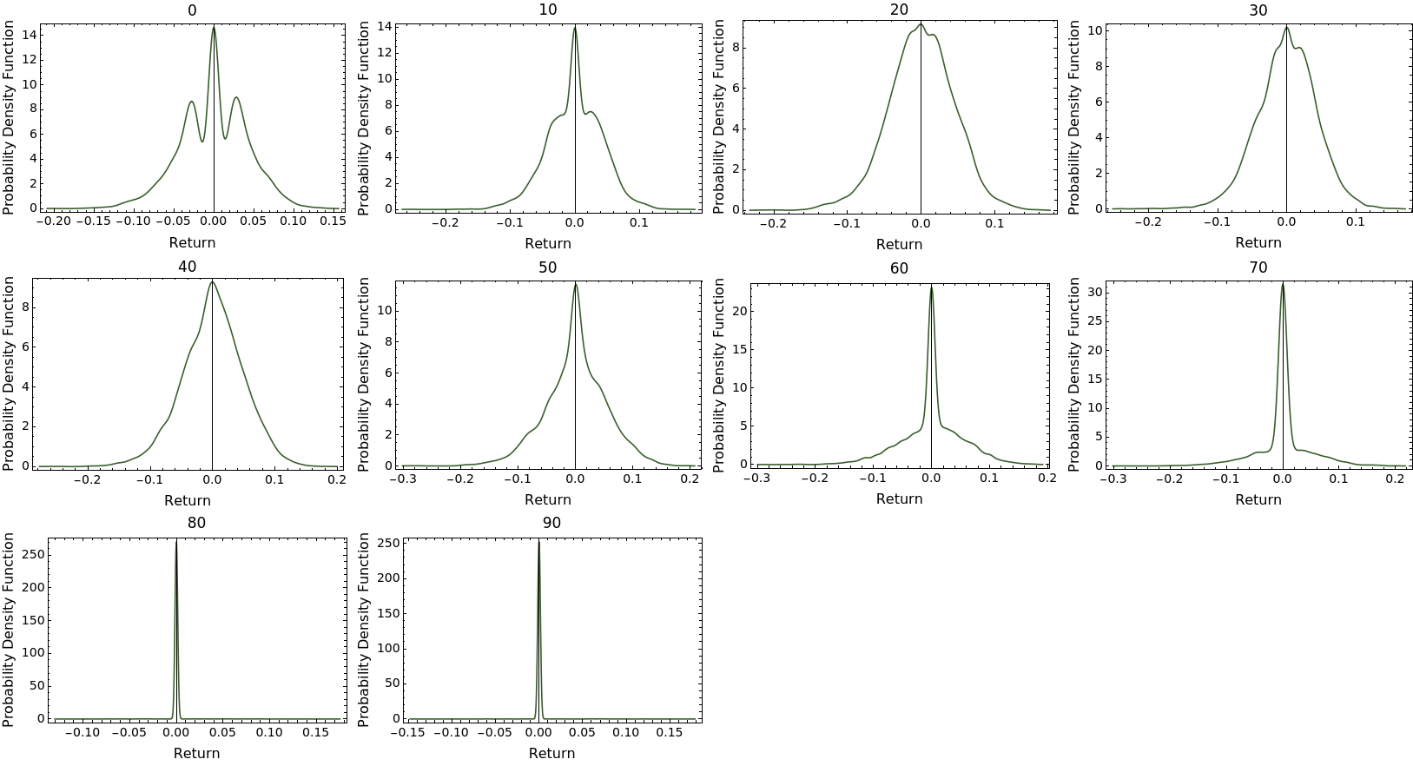
\includegraphics[scale=0.2]{img/dist_prices.png} \end{figure}\markdownRendererInterblockSeparator
{}\markdownRendererHorizontalRule{}\markdownRendererInterblockSeparator
{}\markdownRendererHeadingFour{This is another sample}\markdownRendererInterblockSeparator
{}\markdownRendererUlBegin
\markdownRendererUlItem Some maths material\markdownRendererUlItemEnd 
\markdownRendererUlEnd \markdownRendererInterblockSeparator
{}\begin{align} A &= U \times S \times V^T\ \sigma &= \frac{x\times y}{\sqrt[3]{\alpha + \beta}} \end{align}\markdownRendererInterblockSeparator
{}\markdownRendererHorizontalRule{}\markdownRendererInterblockSeparator
{}\markdownRendererHeadingFour{\markdownRendererCodeSpan{pipeTables} and \markdownRendererCodeSpan{tableCaptions}}\markdownRendererInterblockSeparator
{}\markdownRendererTable{Demonstration of pipe table syntax.}{4}{4}{rldc}%
{{Right}%
{Left}%
{Default}%
{Center}%
}%
{{12}%
{12}%
{12}%
{12}%
}%
{{123}%
{123}%
{123}%
{123}%
}%
{{1}%
{1}%
{1}%
{1}%
}%
\markdownRendererInterblockSeparator
{}\markdownRendererHorizontalRule{}\relax